\chapter{Sistemi lineari}
\lecture{4}{25 Nov. 12:11}{Richiami}
\section{Relazioni di equivalenza}

Una relazione si dice di equivalenza se gode di tutte e tre le
seguenti proprietà:

\begin{itemize}
  \item{\makebox[4cm]{Proprietà Riflessiva\hfill}
    \makebox[4cm]{$\forall a\in S\phantom{.}$\hfill} $a\sim a$}
  \item{\makebox[4cm]{Proprietà Simmetrica\hfill}
    \makebox[4cm]{$\forall a\sim b\phantom{.}$\hfill} $b\sim a$}
  \item{\makebox[4cm]{Proprietà Transitiva\hfill}
      \makebox[4cm]{$\forall a\sim b, \forall b\sim
    c\phantom{.}$\hfill} $a\sim c$}
\end{itemize}

\begin{nota}
  \phantom{text}
  \leavevmode\\
  \begin{itemize}
    \item[]{\makebox[2cm]{$a\sim b$\hfill}     $a \text{ è in relazione a }b$}
    \item[]{\makebox[2cm]{$a\nsim b$\hfill}   $a \text{ non è in
      relazione con }b$}
    \item[]{\makebox[2cm]{$\sum$\hfill}     $\text{Insieme dei
      segmenti orientati (Coppia ordinata di punti A;B)}$}
  \end{itemize}
\end{nota}

\begin{align*}
  AB=CD\Leftrightarrow
  &A=C \\
  &B=D
\end{align*}

\begin{align*}
  AB=BA\Leftrightarrow
  &A=B \text{ (segmento orientato nullo)}
\end{align*}

\begin{align*}
  AB\sim CD\Leftrightarrow
  \begin{cases}
    \text{Se } A=B\Rightarrow 		& C=D \text{ Tutti i segmenti nulli
    sono equipollenti}\\
    \text{Se } A\neq B\Rightarrow 	& AB \text{ Equipollente a } CD\\
    								& \text{Hanno la stessa lunghezza } |AB|=|CD|\\
    								& \text {Hanno la stessa direzione } \overrightarrow{r}_{AB}=\overrightarrow{r}_{CD}\\
    								&\text{Hanno lo stesso verso}
  \end{cases}
\end{align*}

\begin{nota}
  \phantom{text}
  \leavevmode\\
  Un vettore è definito come un'entità che ha una \textbf{direzione}
  e un \textbf{verso}, oltre a una \textbf{modulo} (o intensità).
  Spesso si confondono i concetti di direzione e verso, ma essi
  rappresentano due aspetti distinti di un vettore.
  \leavevmode\\\\
  \highlight{\text{Direzione}}
  \leavevmode\\
  La \textbf{direzione} di un vettore è la retta lungo cui il vettore
  agisce. Due vettori hanno la stessa direzione se sono paralleli o
  giacciono sulla stessa linea, indipendentemente dal verso in cui
  puntano. In altre parole, la direzione specifica l'orientamento del
  vettore nello spazio senza considerare il verso in cui punta.
  \leavevmode\\\\
  \highlight{\text{Verso}}
  \leavevmode\\
  Il \textbf{verso} di un vettore, invece, indica il senso in cui il
  vettore punta lungo la sua direzione. Per esempio, lungo una data
  retta, un vettore può puntare in due sensi opposti: verso destra o
  verso sinistra, verso l'alto o verso il basso, a seconda del
  sistema di riferimento utilizzato. Il verso distingue quindi tra le
  due possibili orientazioni lungo la direzione del vettore.
  \leavevmode\\\\
  \highlight{\text{Esempio Grafico}}
  \leavevmode\\
  Nel seguente esempio, i vettori \(\vec{A}\) e \(\vec{B}\) hanno la
  stessa direzione, ma versi opposti. La loro direzione è la stessa
  retta, ma \(\vec{A}\) punta verso destra, mentre \(\vec{B}\) punta
  verso sinistra.
  \leavevmode\\
  \begin{center}
    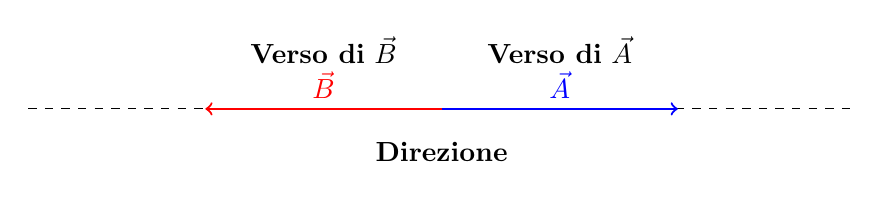
\begin{tikzpicture}[scale=1.5]
      % Disegno della direzione come linea tratteggiata
      \draw[dashed] (-3.5,0) -- (3.5,0);

      % Vettore A
      \draw[->, thick, blue] (0,0) -- (2,0) node[midway, above] {$\vec{A}$};

      % Vettore B
      \draw[<-, thick, red] (-2,0) -- (0,0) node[midway, above] {$\vec{B}$};

      % Etichette per la direzione e verso
      \node[above] at (1, 0.3) {\textbf{Verso di} $\vec{A}$};
      \node[above] at (-1, 0.3) {\textbf{Verso di} $\vec{B}$};
      \node[below] at (0, -0.2) {\textbf{Direzione}};
    \end{tikzpicture}
  \end{center}
  \leavevmode\\
  In questo esempio:
  \begin{itemize}
    \item \textbf{Direzione:} Entrambi i vettori \(\vec{A}\) e
      \(\vec{B}\) giacciono sulla stessa retta (la linea
      tratteggiata) e hanno la stessa direzione.
    \item \textbf{Verso:} Il vettore \(\vec{A}\) punta verso destra,
      mentre il vettore \(\vec{B}\) punta verso sinistra, quindi i
      due vettori hanno versi opposti.
  \end{itemize}
\end{nota}
\leavevmode\\\\
$AB=\{\text{Tutti i segmenti orientati, equipollenti ad }AB\}=\text{Vettore geometrico}$
\leavevmode\\\\
$\overrightarrow{AB}=\overrightarrow{CD}\Leftrightarrow AB\sim CD$
\leavevmode\\\\
$\overrightarrow{AB}+\overrightarrow{CD}=\overrightarrow{AB}+\overrightarrow{BE}=\overrightarrow{AE}\sim\text{Vettore geometrico rappresentato dal segmento orientato AE}$

\section{La somma Vettoriale è un gruppo Abeliano}

$\overrightarrow{AB}+\overrightarrow{BB}=\overrightarrow{AB}$

\begin{nota}
  $\overrightarrow{BB}$ Vettore geometrico nullo
\end{nota}
\leavevmode\\
$\overrightarrow{AB}+\overrightarrow{BA}=\overrightarrow{AA}$
\leavevmode\\
\begin{nota}
  $\overrightarrow{BA}$ Vettore geometrico opposto
\end{nota}
\leavevmode\\
\begin{wrapfigure}{r}{7cm}
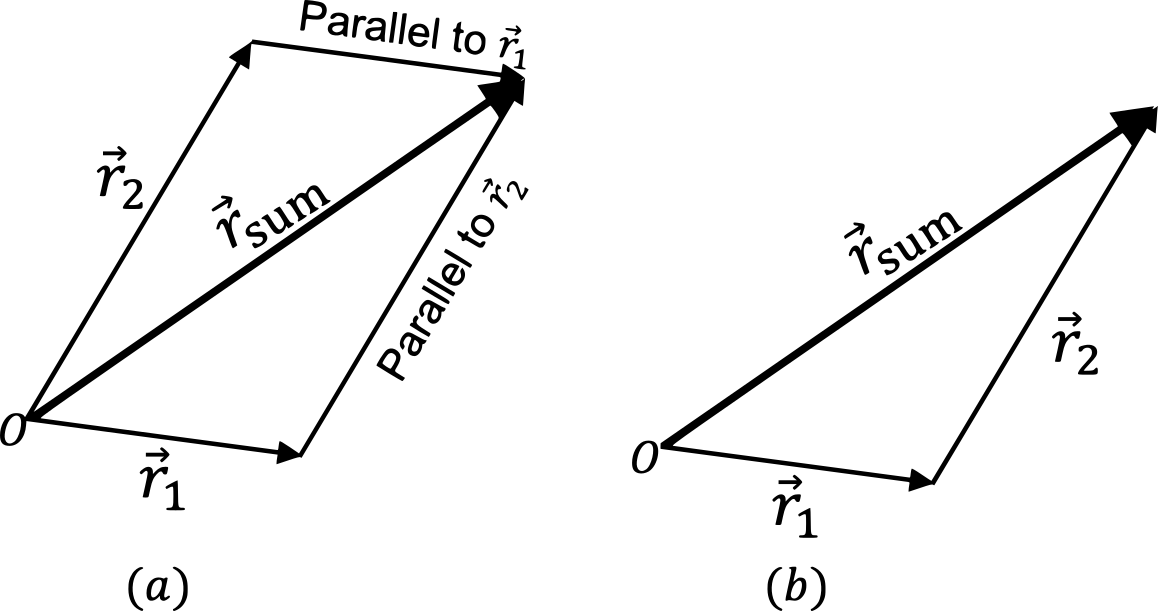
\includegraphics[height=0.28\textwidth]{Figures/somma tra vettori.pdf}
\end{wrapfigure} 

$\overrightarrow{U}+\overrightarrow{V}=\overrightarrow{V}+\overrightarrow{U}$
\leavevmode\\
\begin{flalign*}
  \overrightarrow{U}=\overrightarrow{AB}   & &\overrightarrow{U}+\overrightarrow{V}=\overrightarrow{AC}
  &&&&&&&&&&&&&&&&&&&&&&&&&&&&&&&&&&\\
  \overrightarrow{V}=\overrightarrow{BC}   &
  \phantom{...}\overrightarrow{V}=\overrightarrow{AD}\Rightarrow
  &\overrightarrow{U}=\overrightarrow{DC}  &&&&&&&&&&&&&&&&&&&&&&&&&&&&&&&&&&\\
  &
  &\overrightarrow{V}+\overrightarrow{U}=\overrightarrow{AC}
  &&&&&&&&&&&&&&&&&&&&&&&&&&&&&&&&&&
\end{flalign*}
\leavevmode\\\\\\\\\\\\
$(\overrightarrow{U}+\overrightarrow{V})+\overrightarrow{W}=\overrightarrow{U}+(\overrightarrow{V}+\overrightarrow{W})$
\leavevmode\\
\begin{flalign*}
	\overrightarrow{U}+\overrightarrow{V}		&=\overrightarrow{AC}	& &&&&&&&&&&&&&&&&&&&&&&&&&&&&&&&&&&&&&&&&&&&&&&&&&&&&&&&&&&&&&&&&&&&&&&&&&&&& \\
	(\overrightarrow{U}+\overrightarrow{W})+\overrightarrow{W}	&=\overrightarrow{AC}+\overrightarrow{CD}	&=\overrightarrow{AD} &&&&&&&&&&&&&&&&&&&&&&&&&&&&&&&&&&&&&&&&&&&&&&&&&&&&&&&&&&&&&&&&&&&&&&&&&&&&
\end{flalign*}

\leavevmode\\
\begin{flalign*}
	\overrightarrow{V}+\overrightarrow{W}		&=\overrightarrow{BD}	& &&&&&&&&&&&&&&&&&&&&&&&&&&&&&&&&&&&&&&&&&&&&&&&&&&&&&&&&&&&&&&&&&&&&&&&&&&&& \\
	\overrightarrow{U}+(\overrightarrow{W}+\overrightarrow{W})	&=\overrightarrow{AB}+\overrightarrow{BD}	&=\overrightarrow{AD} &&&&&&&&&&&&&&&&&&&&&&&&&&&&&&&&&&&&&&&&&&&&&&&&&&&&&&&&&&&&&&&&&&&&&&&&&&&&
\end{flalign*}

\begin{align*}
	\beta\cdot \overrightarrow{u}
	\begin{cases}
		\text{Se } \beta=0 \text{ o } \overrightarrow{u}=0 \Rightarrow& \overrightarrow{0}\\
		\text{Se } \beta\neq0 \text{ e } \overrightarrow{u}\neq 0 \Rightarrow& \text{ Stessa direzione di }\overrightarrow{u}\\
		\text{Se e solo se } \beta\neq0 \Rightarrow& \text{Stesso verso di } \overrightarrow{u}
	\end{cases}\\
	\beta\in\mathbb{R}
\end{align*}

$$|\beta\cdot\overrightarrow{u}|=|\beta|\cdot|\overrightarrow{u}|$$